% Created 2023-12-05 Tue 12:04
% Intended LaTeX compiler: pdflatex
\documentclass[12pt, a4paper]{article}
\usepackage[utf8]{inputenc}
\usepackage[T1]{fontenc}
\usepackage{graphicx}
\usepackage{longtable}
\usepackage{wrapfig}
\usepackage{rotating}
\usepackage[normalem]{ulem}
\usepackage{amsmath}
\usepackage{amssymb}
\usepackage{capt-of}
\usepackage{hyperref}
\usepackage{placeins}
\usepackage{gensymb}
\usepackage[letterpaper]{geometry}
\geometry{top=1.0in, bottom=1.0in, left=1.0in, right=1.0in}
\usepackage{rotating}
\usepackage{graphicx}
\usepackage{pgfplots}
\usepackage{filecontents}
\usepackage{tikz}
\usepackage{fancyhdr}
\usepackage{enumitem}
\pagestyle{fancy}
\lhead{}
\chead{}
\rhead{Johnson \thepage}
\lfoot{}
\cfoot{}
\rfoot{}
\renewcommand{\headrulewidth}{0pt}
\renewcommand{\footrulewidth}{0pt}
\setlength\headsep{0.333in}
\newcommand{\bibent}{\noindent \hangindent 40pt}
\newenvironment{workscited}{\newpage \begin{center} Works Cited \end{center}}{\newpage }
\graphicspath{ {./attachments/} }
\author{Christian}
\date{\today}
\title{}
\hypersetup{
 pdfauthor={Christian},
 pdftitle={},
 pdfkeywords={},
 pdfsubject={},
 pdfcreator={Emacs 28.2.50 (Org mode 9.7-pre)}, 
 pdflang={English}}
\begin{document}

\begin{document}
\begin{flushleft}
Christian Johnson\\
\vspace{2mm}Dr. Paul Crilly\\
\vspace{2mm}Antennas and Propogation\\
\vspace{2mm}December 05 2023\\
\vspace{4mm}\begin{center}
Lab 8 Revision
\end{center}
\vspace{1mm}\setlength{\parindent}{0.5in}

In the initial rendition of this lab report, a miscalculation in the polar plot led to inaccuracies in the representation of the Yagi antenna's radiation pattern. Specifically, an oversight in normalizing the gain values resulted in an unintended placement of the maximum gain. This basic revision aims to address this discrepancy by presenting a corrected polar plot with normalized gain values, offering a more accurate depiction of the antenna's directional characteristics. The focus of this revision is on rectifying the earlier error and providing a succinct overview of the improved interpretation.
\section*{Testing Results:}
\label{sec:orgb418610}

Utilizing the Agilent 9912A Field Fox Analyzer, the constructed Yagi antenna underwent testing on the football field. The antenna was rotated in a complete circle at intervals of 45 degrees, and the Signal-to-Noise Ratio (SNR) results were recorded:

\begin{center}
\begin{tabular}{rl}
Normalized Gain (dB) & Azimuth\\[0pt]
8.5 & 0 degrees\\[0pt]
3.5 & 45 degrees\\[0pt]
0 & 90 degrees\\[0pt]
7 & 135 degrees\\[0pt]
6 & 180 degrees\\[0pt]
0.5 & 225 degrees\\[0pt]
2.5 & 270 degrees\\[0pt]
5.5 & 315 degrees\\[0pt]
\end{tabular}
\end{center}

\begin{figure}[htb]
\centering
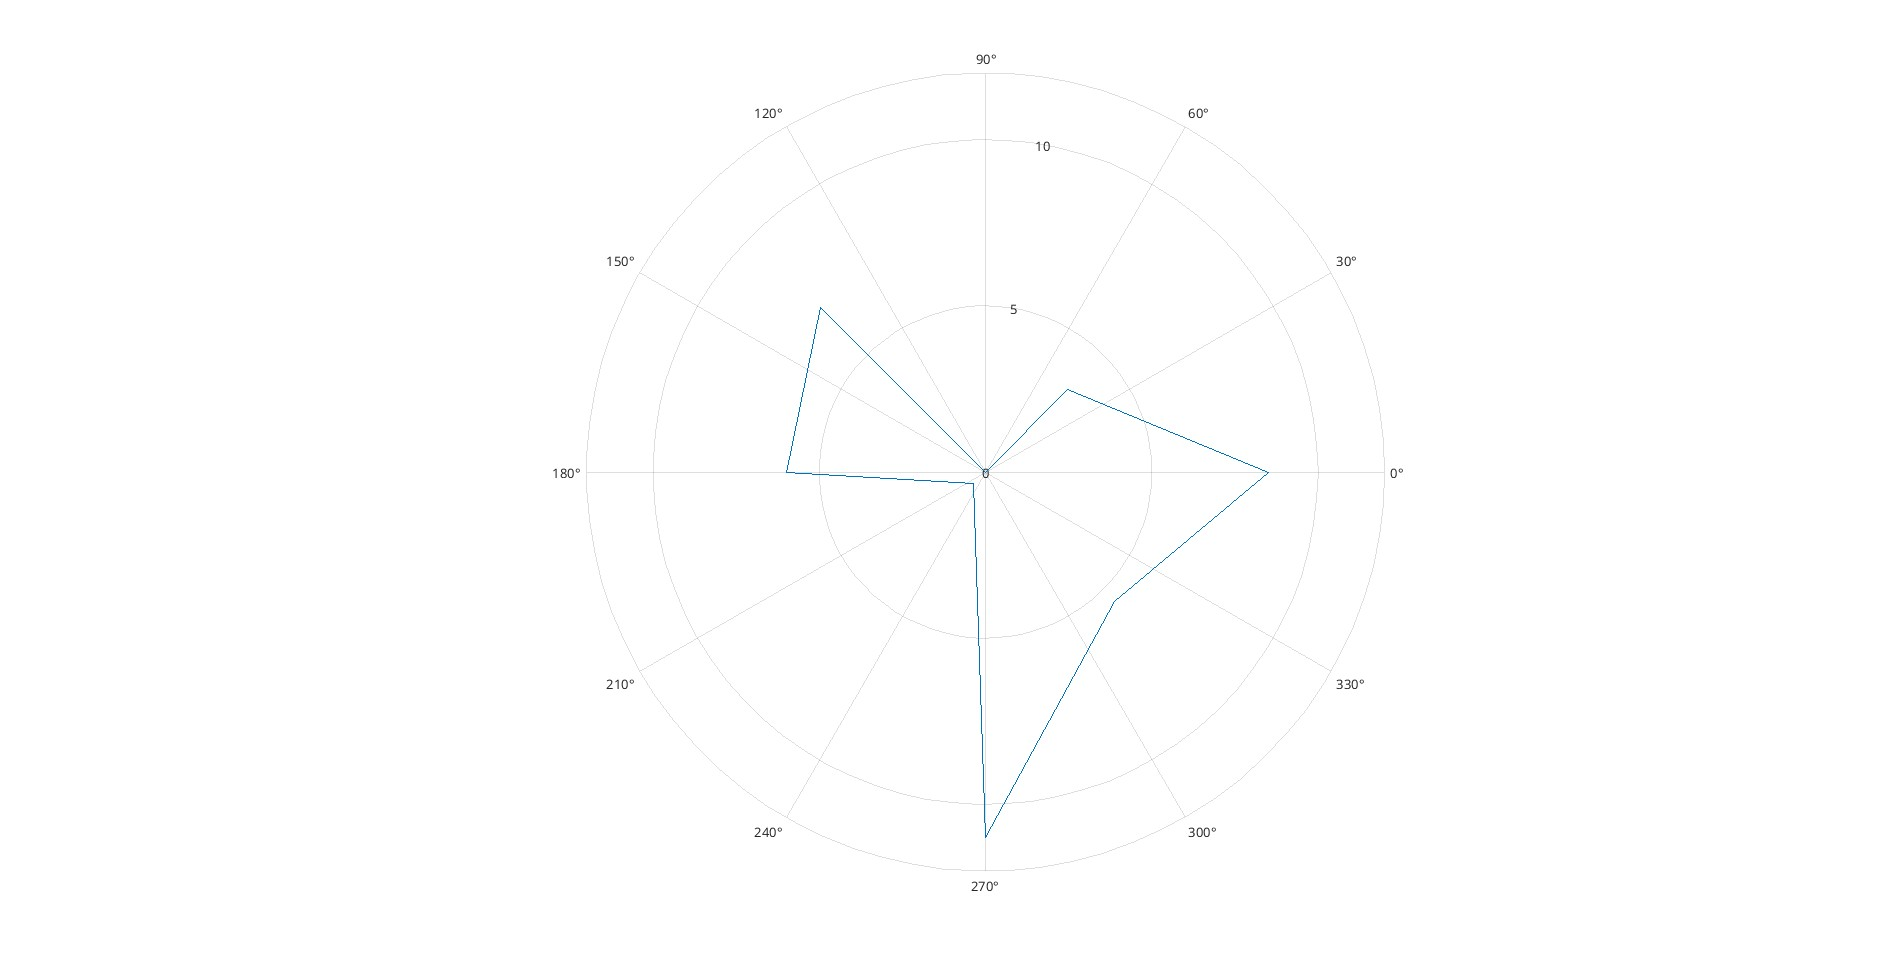
\includegraphics[width=0.7\textwidth]{Polarplot-new.jpg}
\caption{Revised Polar Plot}
\end{figure}


The polar plot has been recalibrated with normalized gain values, showcasing a significantly improved representation of the antenna's radiation pattern. Notably, the maximum gain now occurs at 0 degrees and 135 degrees, aligning more closely with the expected performance. The vaguely lobe-shaped structure with a distinct front and back portion suggests a directional pattern, indicating an enhanced understanding of the antenna's behavior.
Revised Conclusion:

The Yagi antenna lab has provided valuable insights into the design, construction, and testing processes. Despite initial challenges with optimizing the radiation pattern, the corrected polar plot demonstrates a more accurate representation of the antenna's directional characteristics. The improved alignment of the maximum gain with the anticipated angles at 0 degrees and 135 degrees signifies a positive adjustment in the design. This revised interpretation reinforces the importance of accurate testing and recalibration in refining antenna performance analysis.

The answers to the some of the questions in the previous lab report reference my previous polar plot.
My new polar plot looks much closer to the simulated version, with clear frontal and rear lobes. The frontal section looks almost identical (or as close as this discrete representation can get) while the rear lobe is slightly shifted to the left. This is likely due to an error when calculating data - my best guess is that we turned farther than 45 degrees for those measurements, skewing the larger magnitude measurements towards the left of the graph. The 3 dB beamwidth appears to occur between 270 degrees and 300 degrees, and 15 degrees and 60 degrees. These are relatively similar to the simulated graph, although the simulated graph featured a wider frontal lobe that made it difficult to find exact points where the SWR approached 1/2 of maximum. 

\end{document}
\end{document}